\subsection{Deuteron Production}

Compared with proton production, deuteron emission is more difficult to reproduce because the emitted particle is composite. In addition to compound and pre-equilibrium emission, the component decompositions may include contributions such as stripping, knock-out and break-up. As a result, the calculated deuteron spectra show more structure than the proton spectra, especially in the intermediate- and high-outgoing-energy regions. For this reason, the mode selection is again based mainly on the shoulder and high-energy tail, rather than only on the low-energy evaporation peak.

\subsubsection*{\ce{^{28}Si}, Benck, 22807.027}

\Epar{$E_n=28.5$ MeV}

\begin{figure}[H]
    \centering
    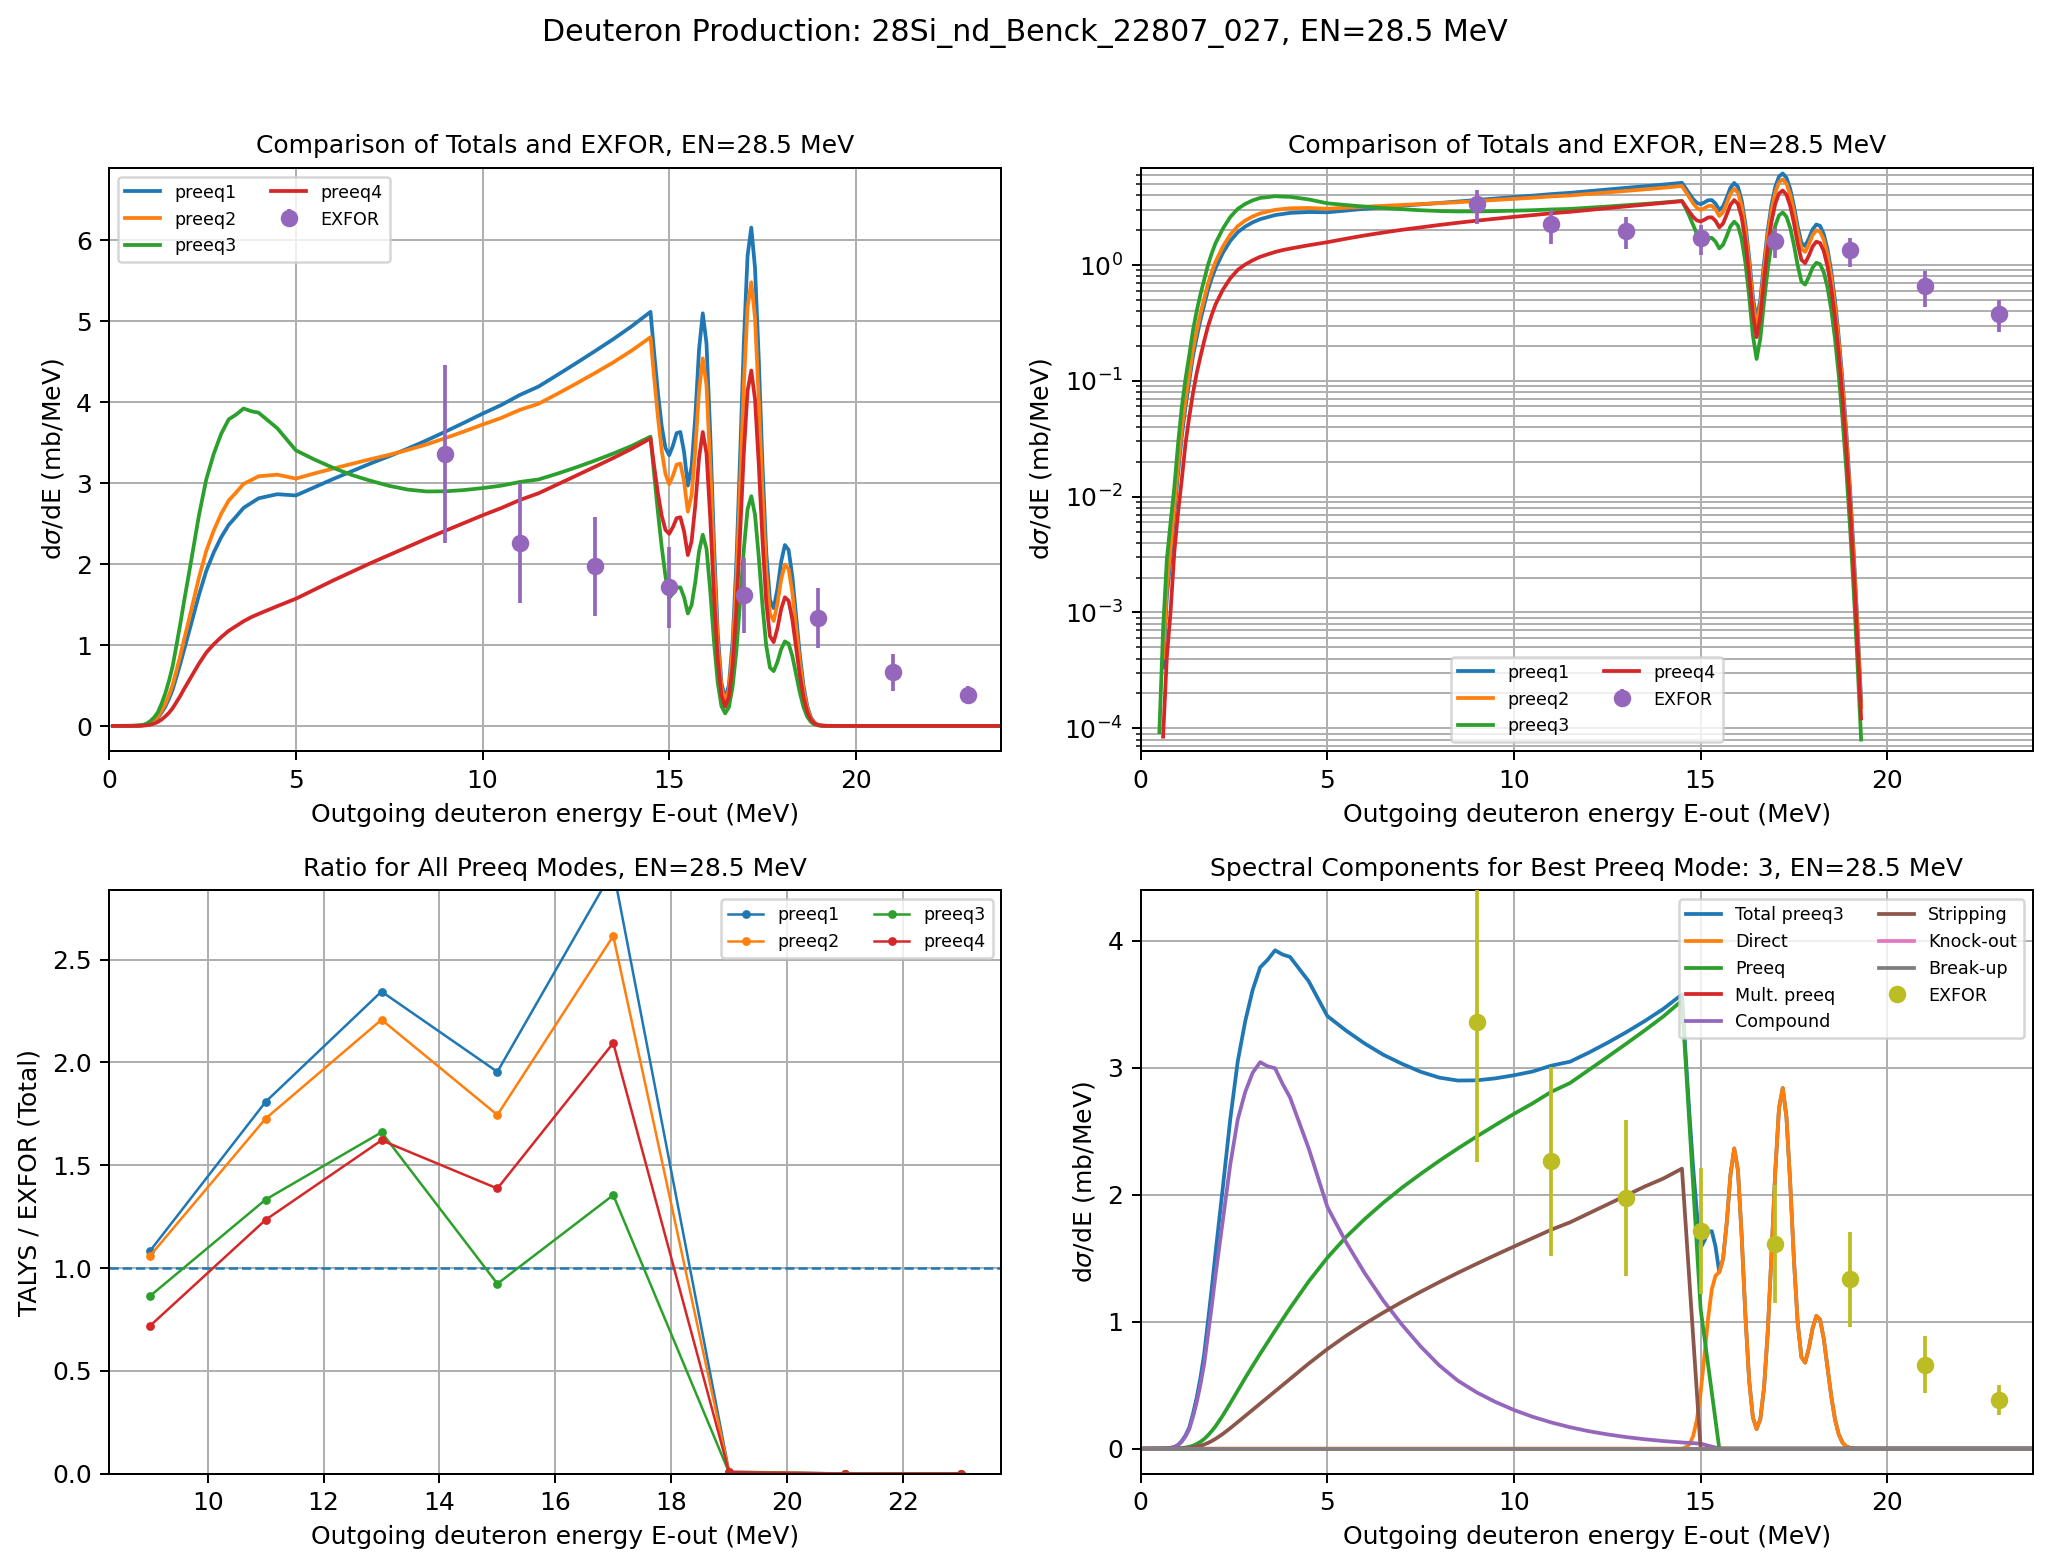
\includegraphics[width=\textwidth]{Images/EN28.5_00_2x2_diagnostics_28Si_nd_Benck_22807_027.png}
    \caption{Diagnostic panels for deuteron production on \ce{^{28}Si} using the Benck EXFOR dataset 22807.027 at $E_n=28.5$ MeV. The decomposition panel corresponds to the selected mode, \texttt{preeqmode=3}.}
    \label{fig:benck-en28p5-d-diagnostics}
\end{figure}

As shown in \cref{fig:benck-en28p5-d-diagnostics}, the deuteron spectrum is less smooth than the corresponding proton-production spectra. The four \texttt{preeqmode} options separate not only in the tail, but also through narrow structures in the mid-to-high outgoing-energy region. This behaviour is consistent with the more complex nature of composite-particle emission, where several mechanisms can contribute to the calculated spectrum.

Among the four options, \texttt{preeqmode=3} gives the most reasonable overall compromise over the better-populated part of the experimental spectrum. The logarithmic panel highlights an important limitation: the TALYS total decreases abruptly around $E_{\mathrm{out}}\approx 19$--20~MeV, while EXFOR still reports non-zero values beyond that region.

The ratio panel confirms this behaviour. After the first points, the ratio fluctuates around $R\simeq 1$, although there is some overprediction in the mid-energy region. The most significant discrepancy occurs above $E_{\mathrm{out}}\sim 19$ MeV, where the TALYS total becomes almost zero while the EXFOR data remain non-zero. This indicates that, for this incident energy, the model has difficulty reproducing the fastest emitted deuterons. The component decomposition shows that, beyond the compound contribution at low $E_{\mathrm{out}}$, the spectrum receives important support from non-compound mechanisms and pre-equilibrium emission in the shoulder region.

\Epar{$E_n=41.0$ MeV}

\begin{figure}[H]
    \centering
    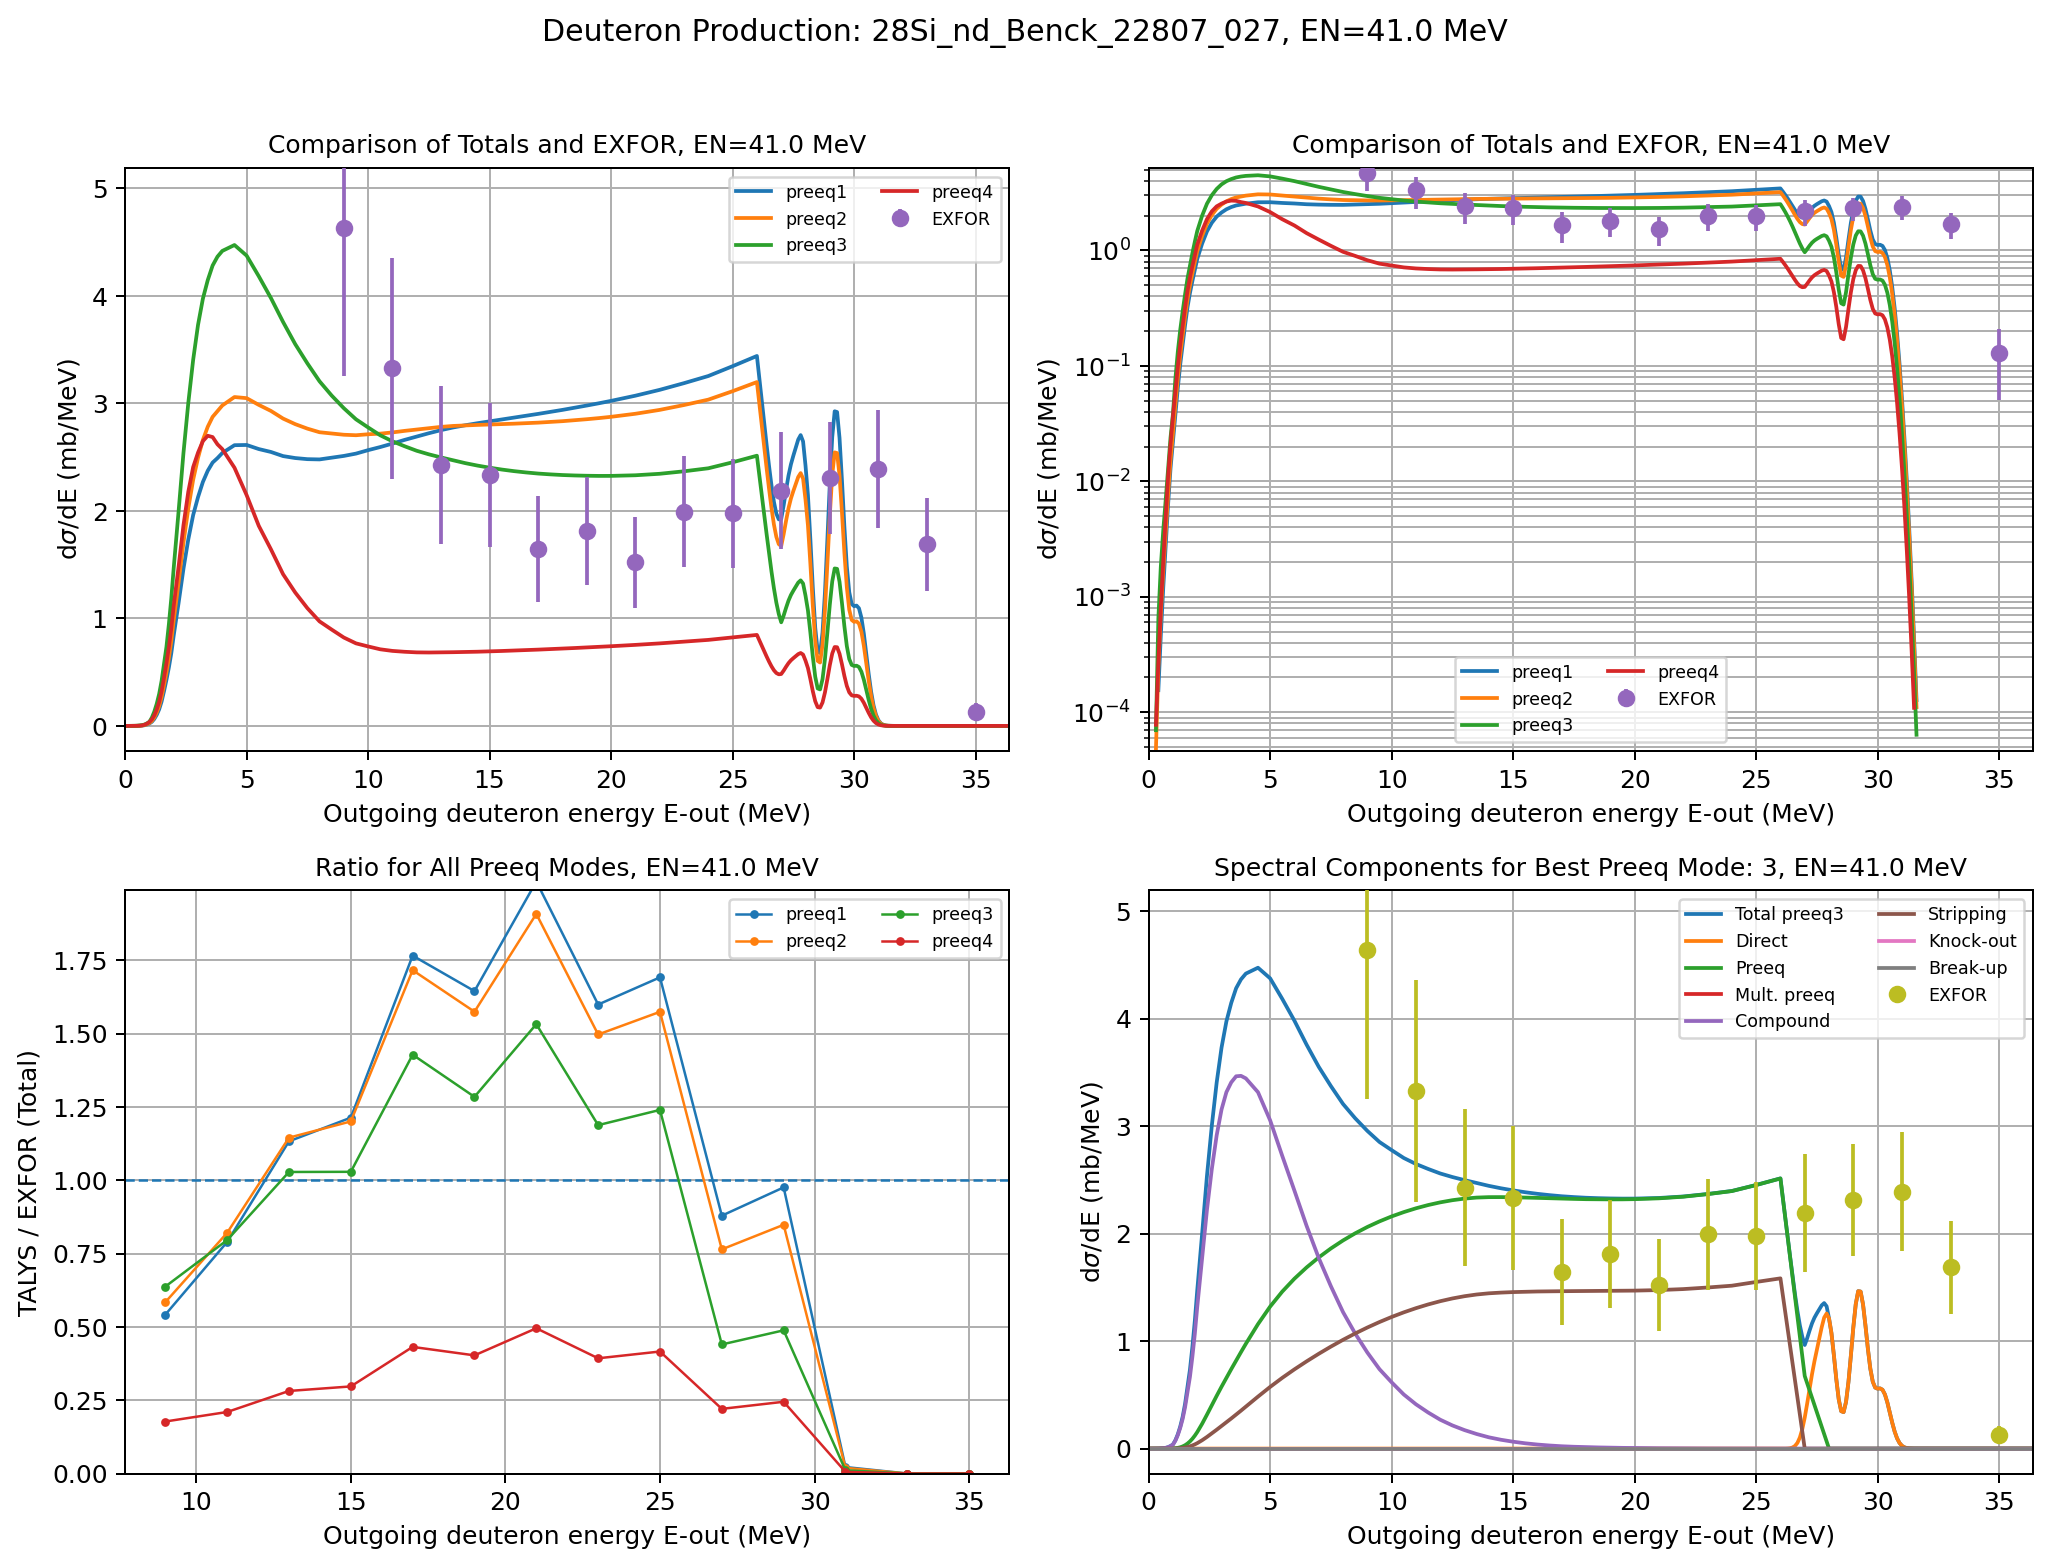
\includegraphics[width=\textwidth]{Images/EN41.0_00_2x2_diagnostics_28Si_nd_Benck_22807_027.png}
    \caption{Diagnostic panels for deuteron production on \ce{^{28}Si} using the Benck EXFOR dataset 22807.027 at $E_n=41.0$ MeV. The decomposition panel corresponds to the selected mode, \texttt{preeqmode=3}.}
    \label{fig:benck-en41-d-diagnostics}
\end{figure}

At $E_n=41.0$ MeV, shown in \cref{fig:benck-en41-d-diagnostics}, the agreement between TALYS and EXFOR improves compared with the lower incident energy. The calculated spectra still show visible structures in the shoulder and high-energy region, but the overall shape follows the experimental trend more coherently.

The ratio panel provides a clearer view of this improvement. Although the ratio still deviates from $R=1$, the decrease is less abrupt than at $E_n=28.5$ MeV. The TALYS prediction only approaches zero above approximately $E_{\mathrm{out}}\sim 30$ MeV. This means that, as the incident energy increases, the region where TALYS remains non-zero extends to higher outgoing energies. Nevertheless, the high-energy tail remains the most problematic region, and \texttt{preeqmode=3} gives the best overall compromise among the tested modes.

\Epar{$E_n=49.0$ MeV}

\begin{figure}[H]
    \centering
    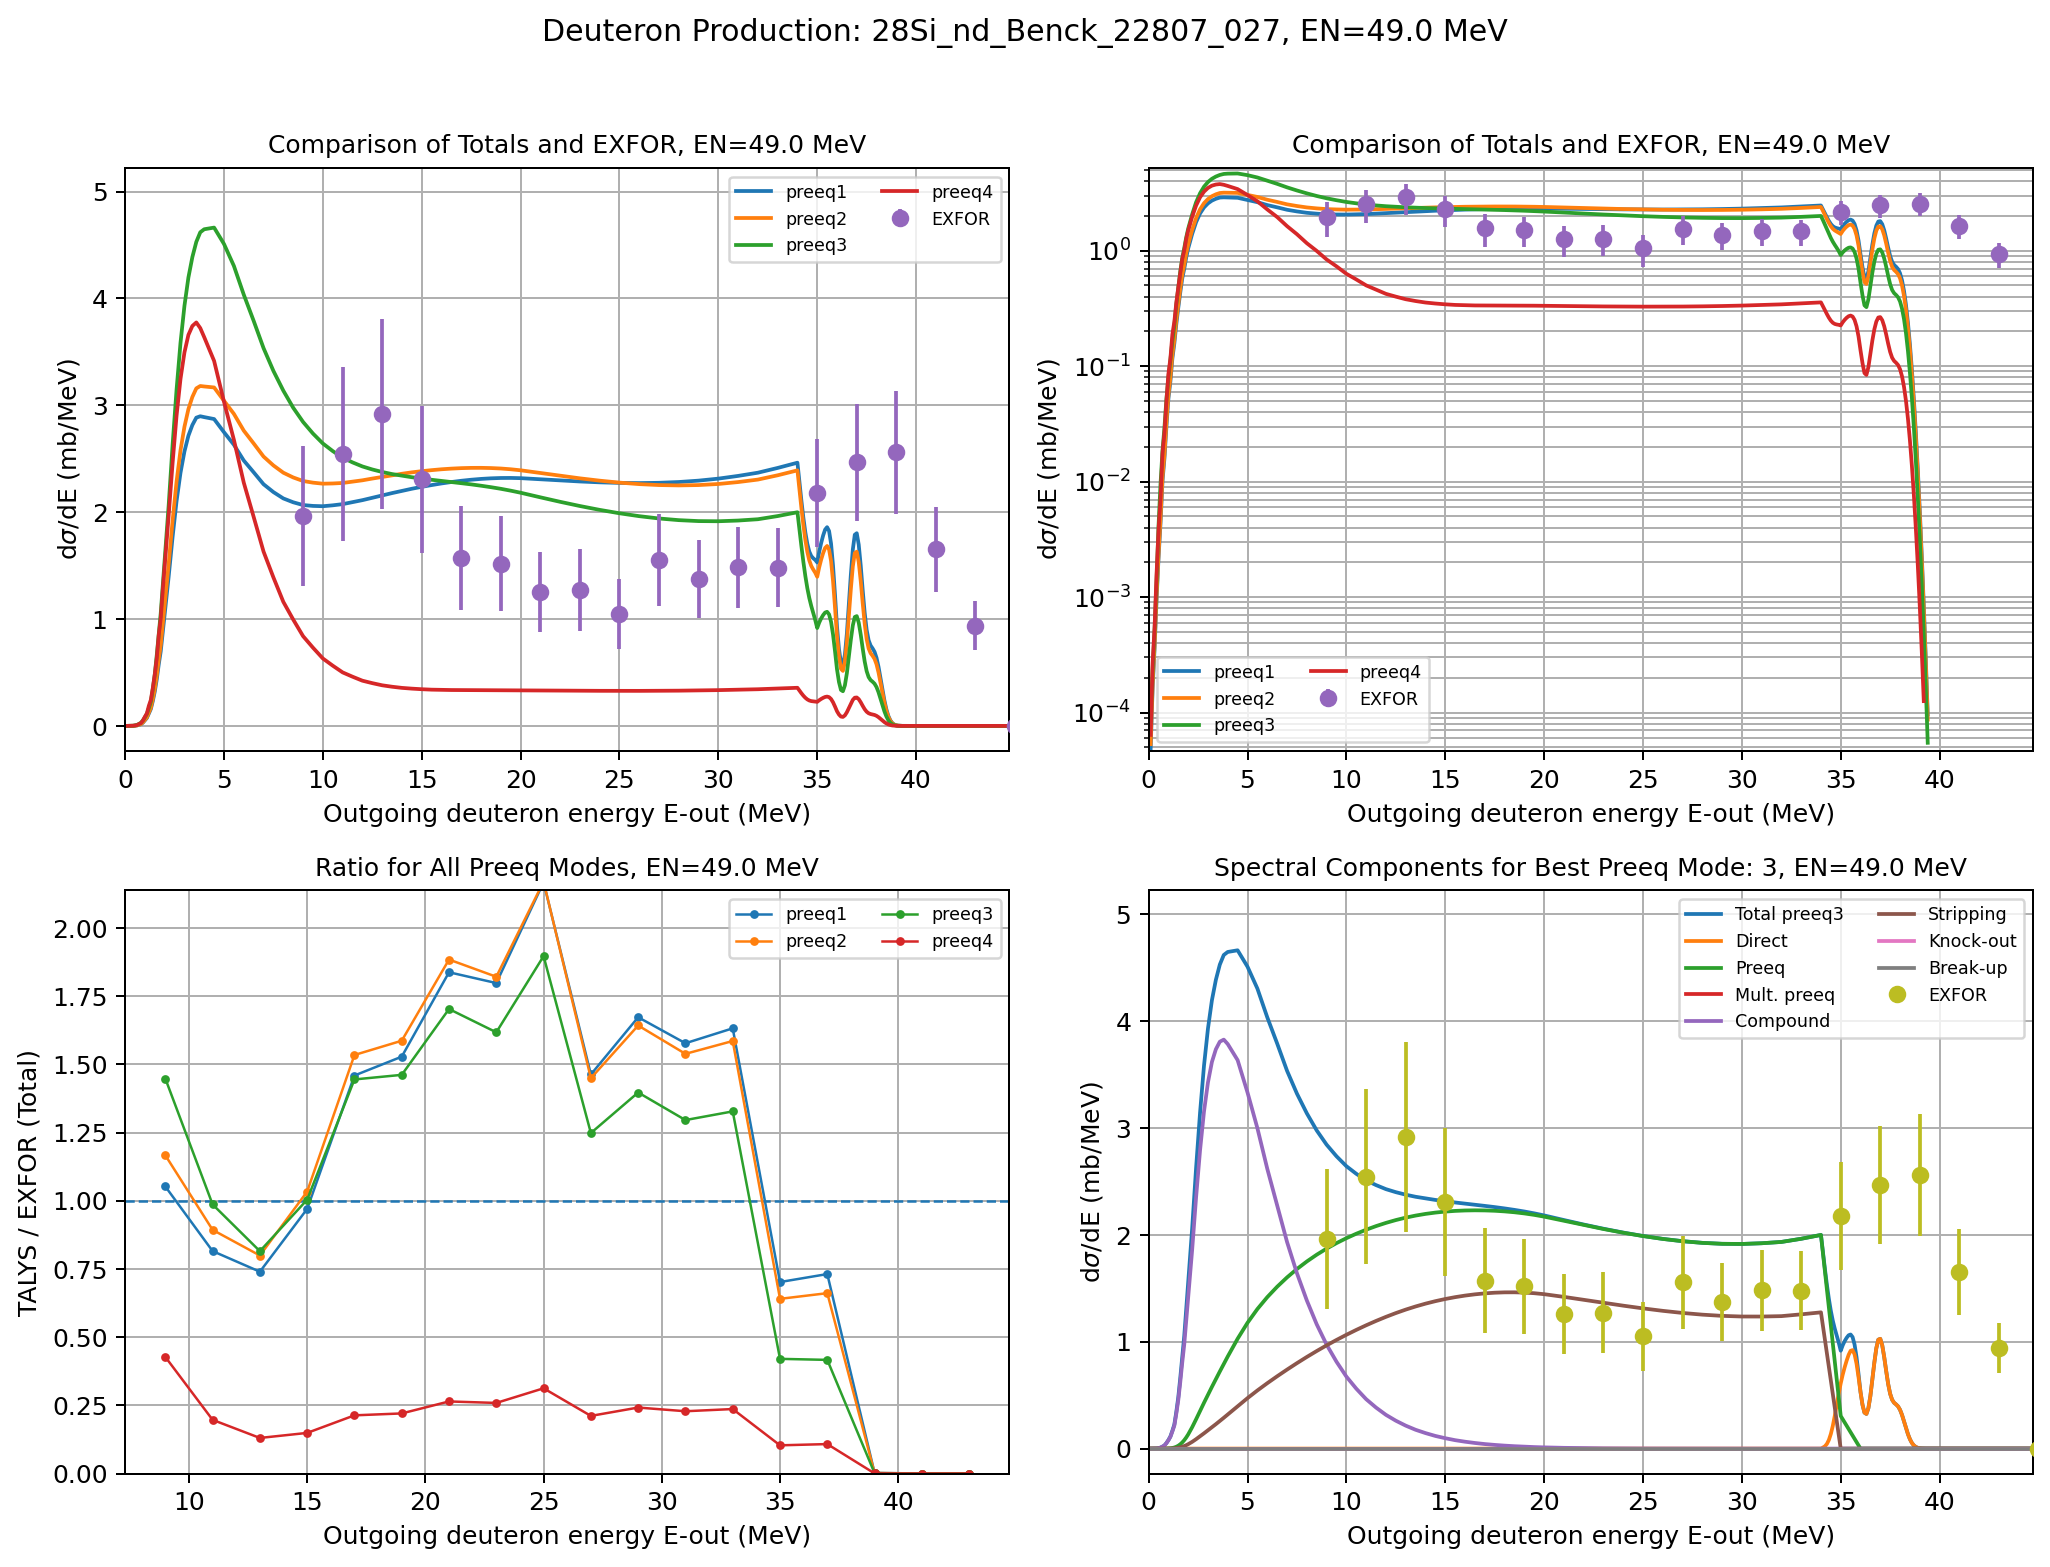
\includegraphics[width=\textwidth]{Images/EN49.0_00_2x2_diagnostics_28Si_nd_Benck_22807_027.png}
    \caption{Diagnostic panels for deuteron production on \ce{^{28}Si} using the Benck EXFOR dataset 22807.027 at $E_n=49.0$ MeV. The decomposition panel corresponds to the selected mode, \texttt{preeqmode=3}.}
    \label{fig:benck-en49-d-diagnostics}
\end{figure}

At $E_n=49.0$ MeV, shown in \cref{fig:benck-en49-d-diagnostics}, the comparison again improves in the sense that the TALYS prediction remains non-zero over a larger outgoing-energy range. The overall overlap between TALYS and EXFOR is better than at lower incident energies, although sizeable discrepancies and experimental error bars remain.

The ratio panel shows that the TALYS prediction falls to nearly zero only around $E_{\mathrm{out}}\sim 39$ MeV. This is a clear shift toward higher outgoing energy compared with the lower incident-energy cases. However, the ratio also shows larger deviations in some regions, meaning that the high-energy end is still difficult to reproduce accurately. For the Benck deuteron-production dataset, the preferred mode is consistently \texttt{preeqmode=3}, but the agreement is still limited by the treatment of the fastest emitted deuterons.

\subsubsection*{\ce{^{28}Si}, Bateman, 13740.006}

Following the same procedure, this dataset was simulated for
$E_n=\{28.0,\,33.0,\,41.0,\,49.0\}\,\mathrm{MeV}$. To keep the report concise and avoid repetition, only
$E_n=\{28.0,\,41.0,\,49.0\}\,\mathrm{MeV}$ are discussed here; the remaining energy is included in Appendix~A.

\Epar{$E_n=28.0$ MeV}

\begin{figure}[H]
    \centering
    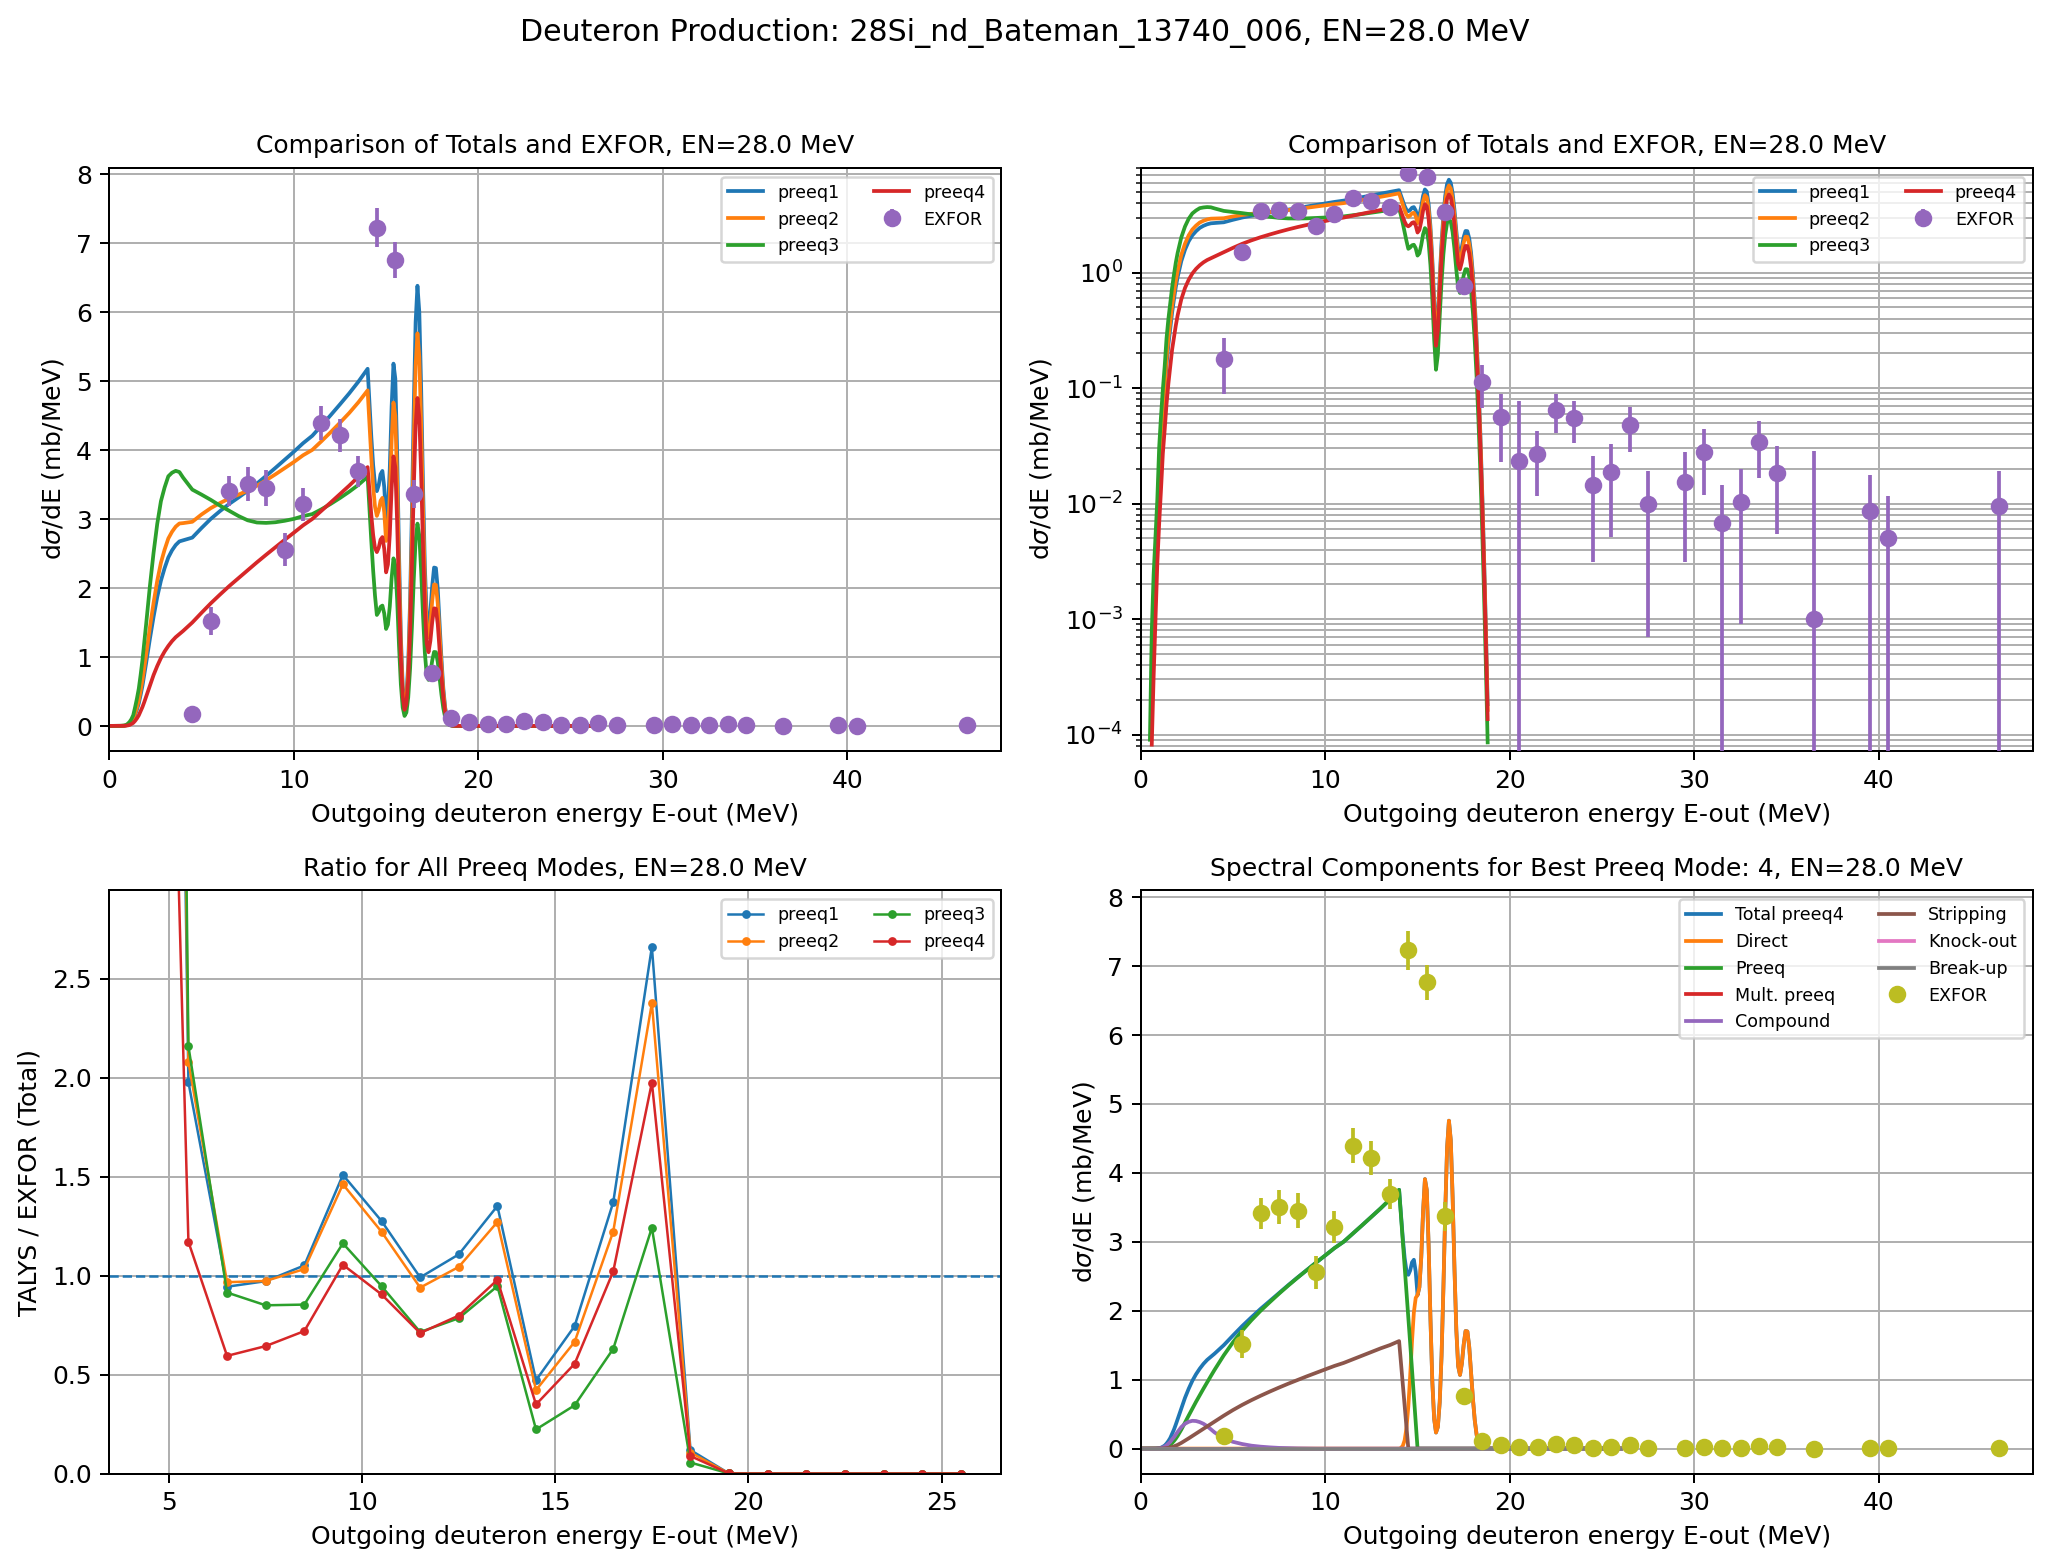
\includegraphics[width=\textwidth]{Images/EN28.0_00_2x2_diagnostics_28Si_nd_Bateman_13740_006.png}
    \caption{Diagnostic panels for deuteron production on \ce{^{28}Si} using the Bateman EXFOR dataset 13740.006 at $E_n=28.0$ MeV. The decomposition panel corresponds to the selected mode, \texttt{preeqmode=4}.}
    \label{fig:bateman-en28-d-diagnostics}
\end{figure}

As shown in \cref{fig:bateman-en28-d-diagnostics}, the Bateman deuteron spectrum also displays a more structured behaviour than the proton-production cases. The \texttt{preeqmode} curves separate not only in the tail, but also through sharp features in the mid-to-high $E_{\mathrm{out}}$ region. Therefore, the mode choice is controlled mainly by the agreement with the EXFOR trend before the TALYS prediction drops to almost zero.

For this incident energy, the selected mode is \texttt{preeqmode=4}. After the first experimental point, which is the most discrepant, the ratio remains closer to $R\simeq 1$ through much of the better-populated region. However, it deviates near the last non-zero TALYS points and eventually collapses to $R\simeq 0$ when the TALYS total becomes almost zero while EXFOR remains non-zero. Thus, at $E_n=28.0$ MeV, the high-energy end is the main limitation of the calculation.

\Epar{$E_n=41.0$ MeV}

\begin{figure}[H]
    \centering
    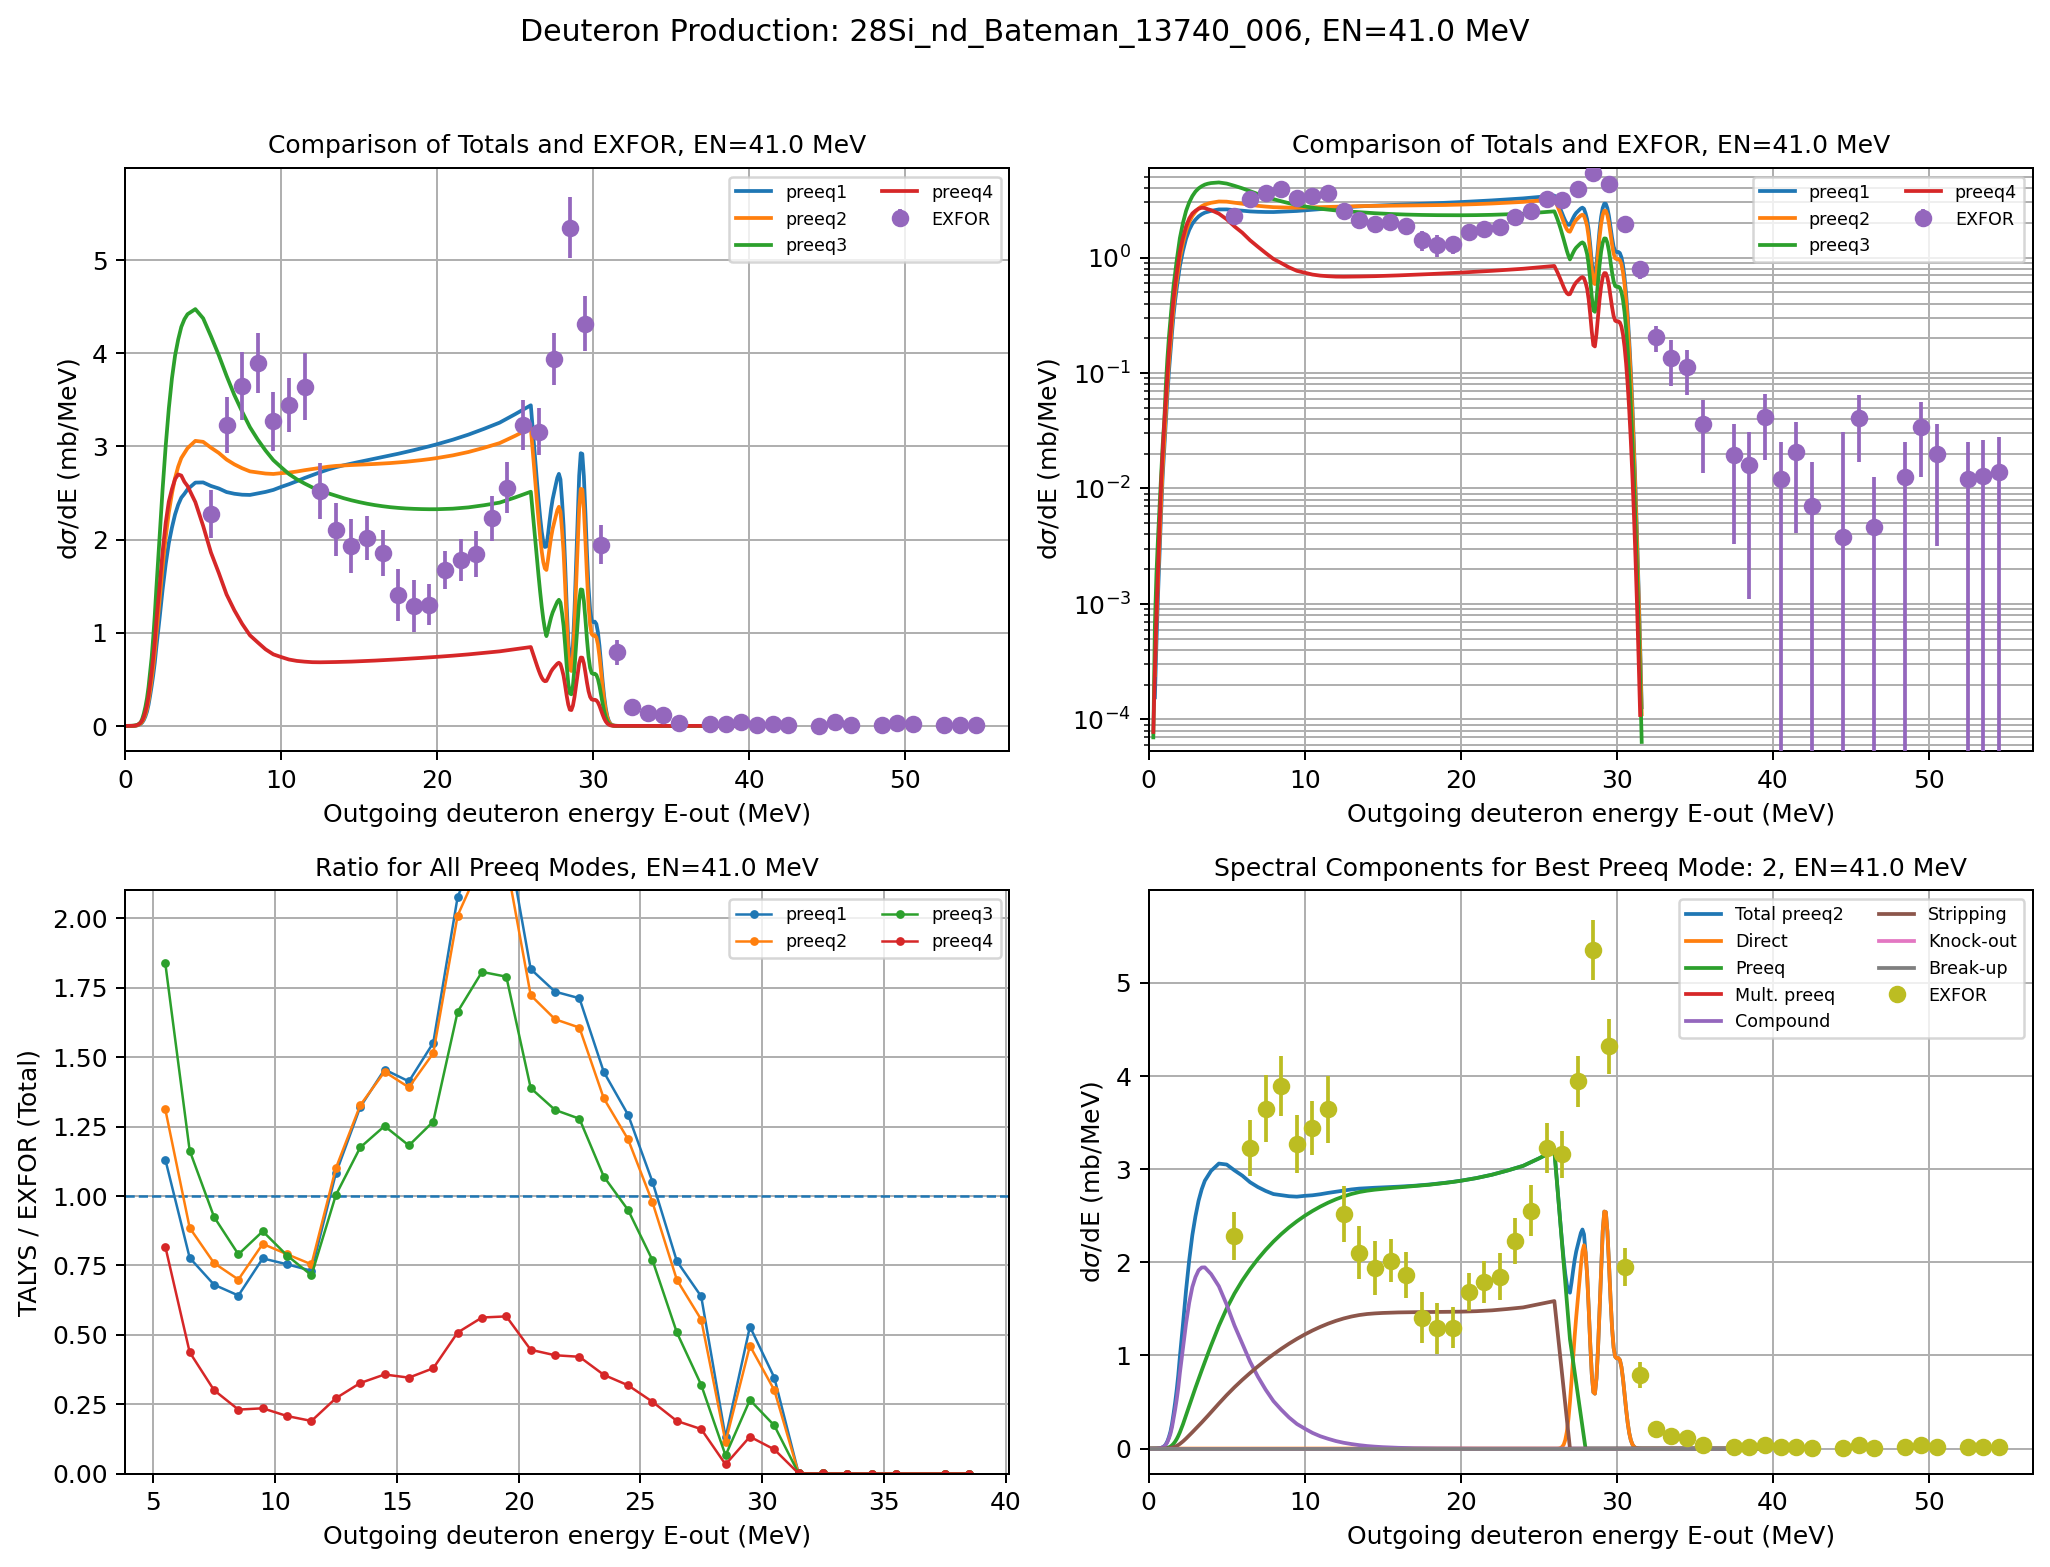
\includegraphics[width=\textwidth]{Images/EN41.0_00_2x2_diagnostics_28Si_nd_Bateman_13740_006.png}
    \caption{Diagnostic panels for deuteron production on \ce{^{28}Si} using the Bateman EXFOR dataset 13740.006 at $E_n=41.0$ MeV. The decomposition panel corresponds to the selected mode, \texttt{preeqmode=2}.}
    \label{fig:bateman-en41-d-diagnostics}
\end{figure}

At $E_n=41.0$ MeV, shown in \cref{fig:bateman-en41-d-diagnostics}, the overall agreement improves, although the calculated spectra still show structured behaviour in the shoulder region. The EXFOR data are followed more coherently over the main part of the measured spectrum, but the high-energy end remains difficult to describe.

For the selected mode, \texttt{preeqmode=2}, the ratio starts close to $R=1$ at lower outgoing energies. It then increases, indicating overprediction in the mid-energy region, before decreasing again and approaching $R\simeq 0$ above $E_{\mathrm{out}}\sim 30$ MeV. Therefore, at this incident energy, the shoulder and high-energy end remain the most sensitive regions for discriminating between modes.

\Epar{$E_n=49.0$ MeV}

\begin{figure}[H]
    \centering
    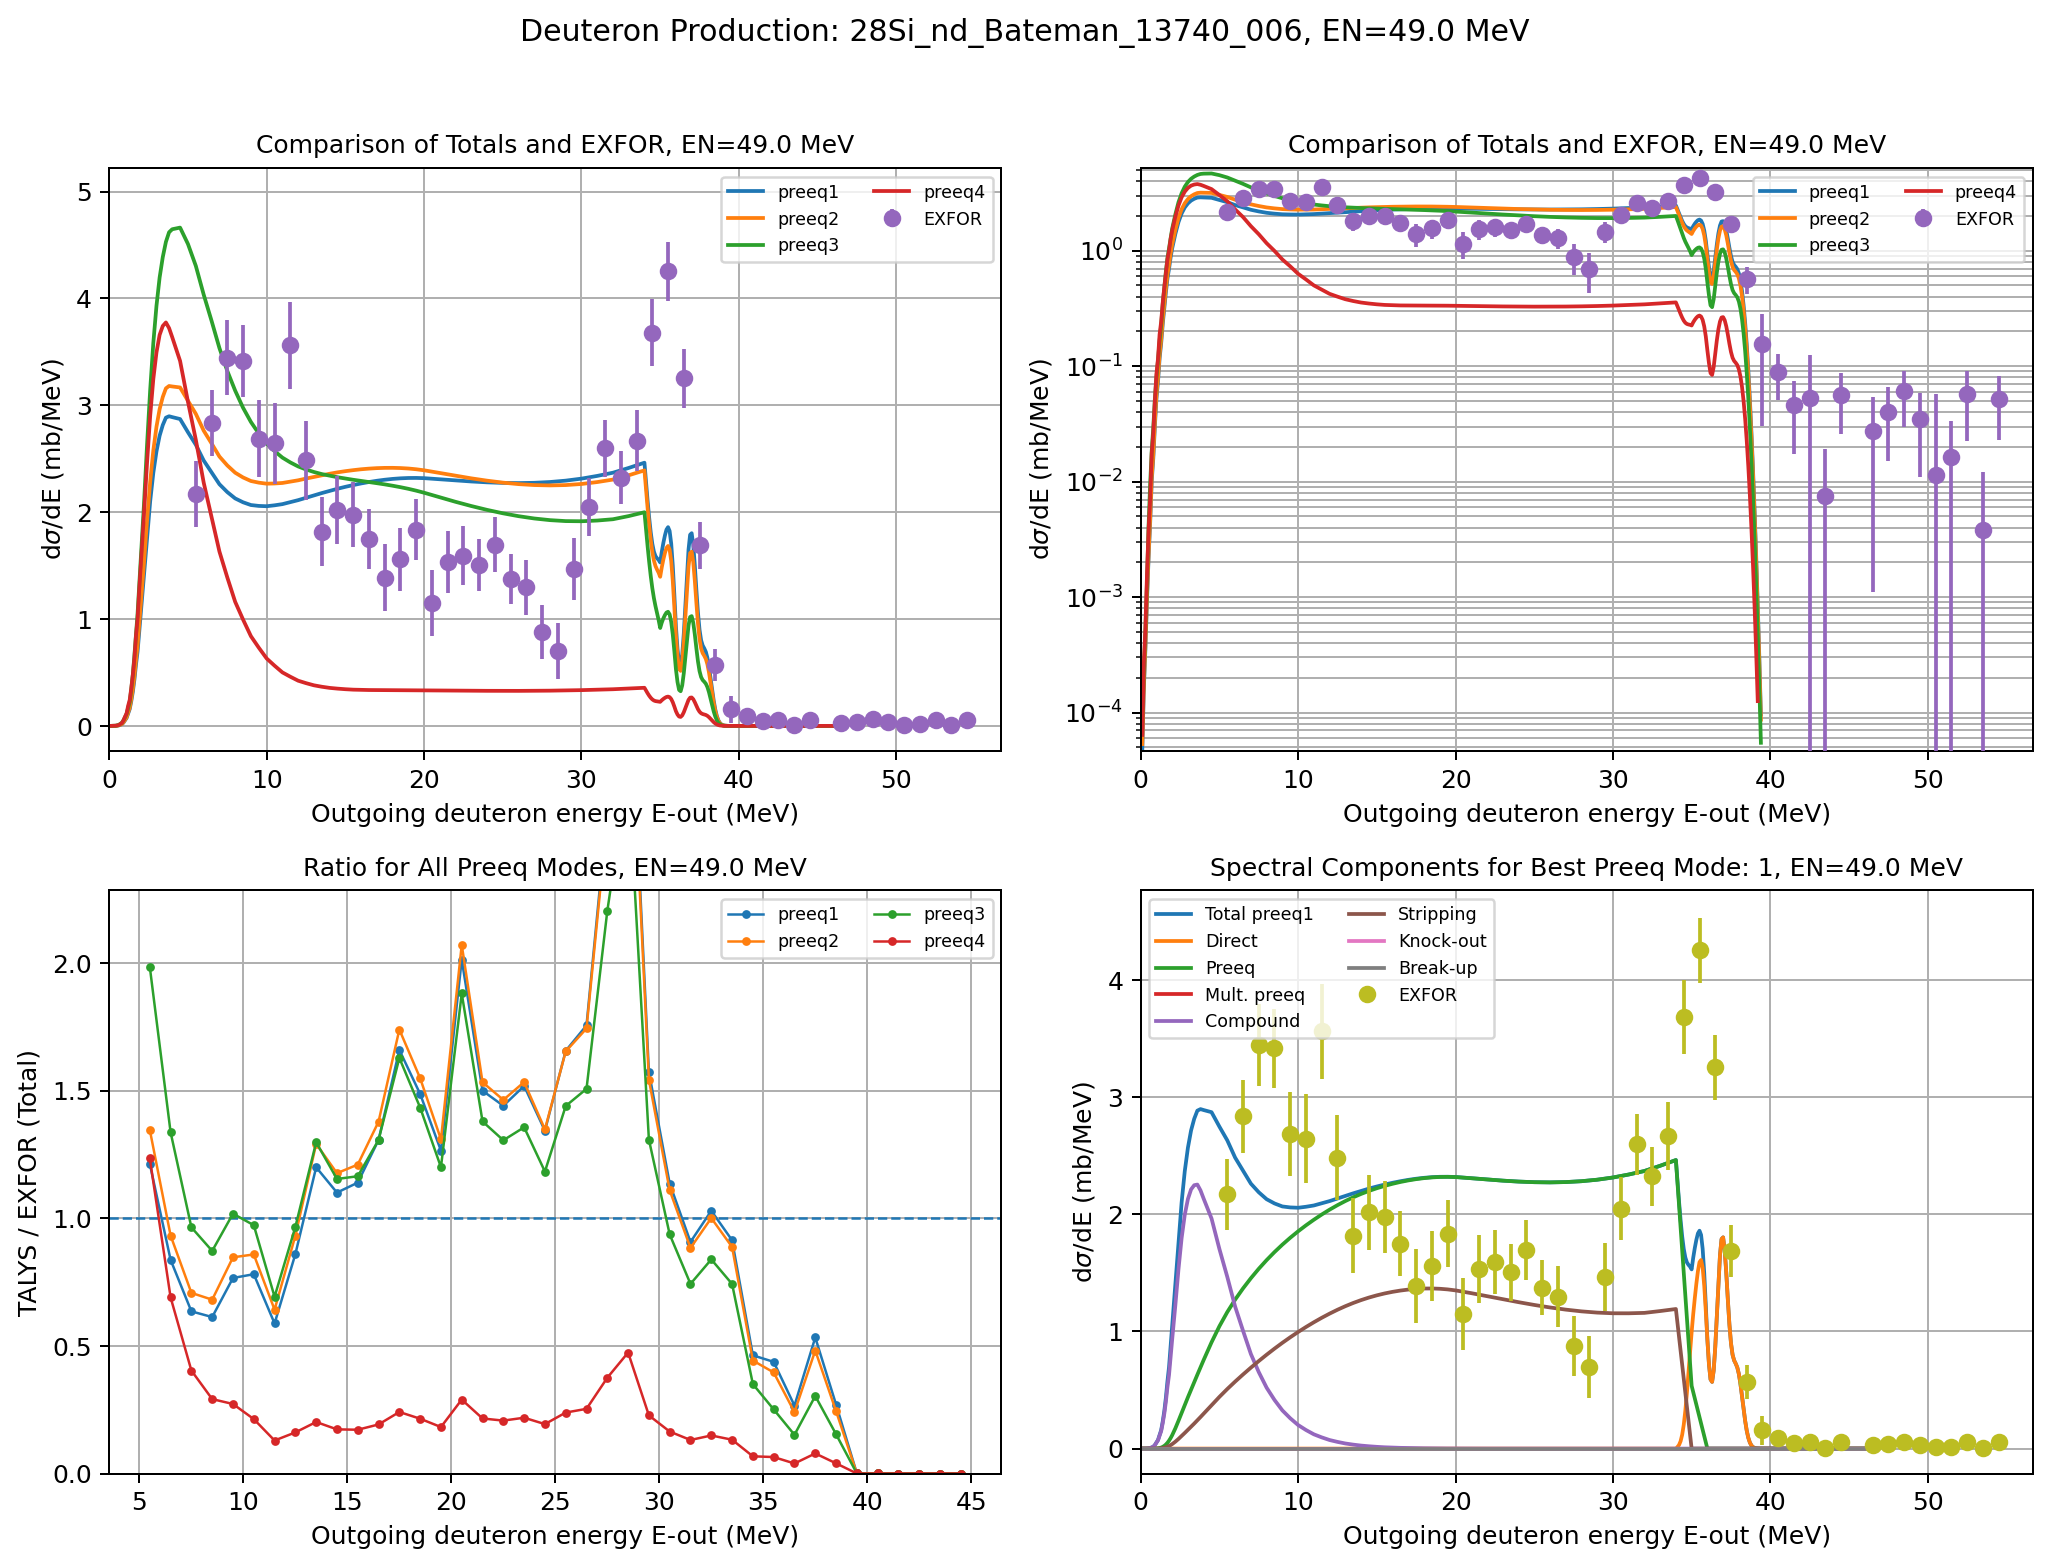
\includegraphics[width=\textwidth]{Images/EN49.0_00_2x2_diagnostics_28Si_nd_Bateman_13740_006.png}
    \caption{Diagnostic panels for deuteron production on \ce{^{28}Si} using the Bateman EXFOR dataset 13740.006 at $E_n=49.0$ MeV. The decomposition panel corresponds to the selected mode, \texttt{preeqmode=1}.}
    \label{fig:bateman-en49-d-diagnostics}
\end{figure}

At $E_n=49.0$ MeV, shown in \cref{fig:bateman-en49-d-diagnostics}, the overlap between TALYS and EXFOR becomes more evident across the main part of the measured spectrum. The spectra still contain narrow structures and the experimental uncertainties remain sizeable, but the general trend is reproduced better than at lower incident energies.

The selected mode changes to \texttt{preeqmode=1}. The ratio panel shows that, over much of the measured interval, this mode remains closer to $R\simeq 1$ than the alternatives. A large ratio peak above 3 is still present, showing that the agreement is not uniform. As in the lower-energy cases, the ratio eventually drops toward $R\simeq 0$, but only at higher $E_{\mathrm{out}}$. This means that the effective high-energy cut-off in the TALYS prediction is shifted to higher outgoing energy as the incident energy increases.

Overall, for the Bateman deuteron-production dataset, the preferred mode is case-dependent: \texttt{preeqmode=4} at $E_n=28.0$ MeV, \texttt{preeqmode=2} at $E_n=41.0$ MeV, and \texttt{preeqmode=1} at $E_n=49.0$ MeV. This confirms that, for deuteron emission, the model choice is controlled mainly by the shoulder and high-energy-tail behaviour rather than by the low-energy evaporation peak.
